\documentclass[12pt]{article}

\usepackage{graphicx}
\usepackage{caption}
\usepackage{amssymb,amsmath,amsthm}




% the following commands set the size of printed page
\setlength{\textheight}{680pt} \setlength{\topmargin}{-50pt}
\setlength{\textwidth}{500pt}
\setlength{\evensidemargin}{-10pt}
\setlength{\oddsidemargin}{-10pt}
%%%%%%%%%%%%%%%%%%%%%%%%%%%%

\begin{document}


\title{Place title of Group Project Here}
\author{Riley Davidson, Laren Edwards, Dallan Olsen, Calix Barrus}

%% comment out next command to put today's date after names of group members, or put a desired day in the parethesis
\date{}

\maketitle

\begin{abstract}
Model the flow of traffic at a stoplight. 
\end{abstract}

%% First Section
\section{Background/Movitation}
Put your background motivation stuff here. You might reference something material here like \cite{ref1}.

%% Second Section 
\section{Modeling Traffic Flow – PDE Approach}

To begin our first foray into modelling traffic flow, we will pull from Volume 4 and work with the given equation for traffic flow $u_t + V_\infty \left(1 - \frac{2u}{u_{\infty}} \right) u_x = 0$. We want to consider three cases:
\begin{enumerate}
    \item What happens to the left of a light after a red light turns green?
    \item What happens before a light when a light turns from green to red? 
    \item What happens both before and after a light when it turns from red to green?
\end{enumerate}

\subsection{Method of Characteristics} 
To begin, we will try to find an explicit solution using the method of characteristics. 

Suppose the solution $u$ is some curve parameterized by $s$ as $u(x(s), t(s))$. Taking the derivative of $u$ with respect to $s$ gives 
\begin{align*} % in the book, the start off with the claim that this equation is = 0 or = f. How do we justify setting u' equal to the differential equation, and also equal to the RHS of the PDE? 
    u'(x(s), t(s)) = \frac{\partial u}{\partial x} \frac{\partial x}{\partial s}  + \frac{\partial u}{\partial t} \frac{\partial t}{\partial s} = u_x \frac{\partial x}{\partial s}  + u_t \frac{\partial t}{\partial s}
\end{align*}
and matching terms with the original differential equation gives us that 
\begin{align*}
    \frac{\partial x}{\partial s}  = V_\infty \left( 1 - \frac{2}{u_\infty} u \right) \\
    \frac{\partial t}{\partial s} = 1 \\
    \frac{\partial u}{\partial s} = 0 .
\end{align*}

Using the fact that $\frac{\partial t}{\partial s} = 1$, we have that 
\begin{align*}
    \frac{\partial x }{\partial t} = V_\infty (1 - \frac{2}{u_\infty} ) \\
    x(t) - x(0) = \int_{0}^{t} V_\infty(1 - \frac{2}{u_\infty} u) dt \\
    x = V_\infty(1 - \frac{2}{u_\infty} u) t + x(0) \\
    t = \frac{1}{  V_\infty(1 - \frac{2}{u_\infty} u) }x - x(0)
\end{align*}
where to evaluate the integral, we used the fact that $\frac{\partial u}{\partial s}$ is $0$, and so the characteristics are constant along the plane. This yields a few cases for the characterstic curves depending on what value of $u$ the curve takes. Based on the physical properties of our model, we have that $u \in [0, u_\infty]$. The slope of the characteristics changed depending on the value of $u$, specifically the slope $m = > 0$ when $u \in [0, \frac{u_\infty}{2}) $, the slope is vertical or undefined when $u = \frac{u_\infty}{2}$, and $m < 0$ when $u \in ( \frac{u_\infty}{2}, u_\infty]$.

Next, suppose that there are some values $x_0, x_1$ from which we draw characteristic curves, and suppose $u(x_0) < u(x_1)$. This will result in shocks, (assuming the shocks happen inside the domain of relevance). See Figures \ref{fig:shock_x1_x2_lt_half}, \ref{fig:shock_x1_x2_gt_half}, and \ref{fig:shock_x1_eq_half} for examples. 

\begin{figure}[!htb]
    \captionsetup{justification=centering}
    \minipage{0.32\textwidth}
    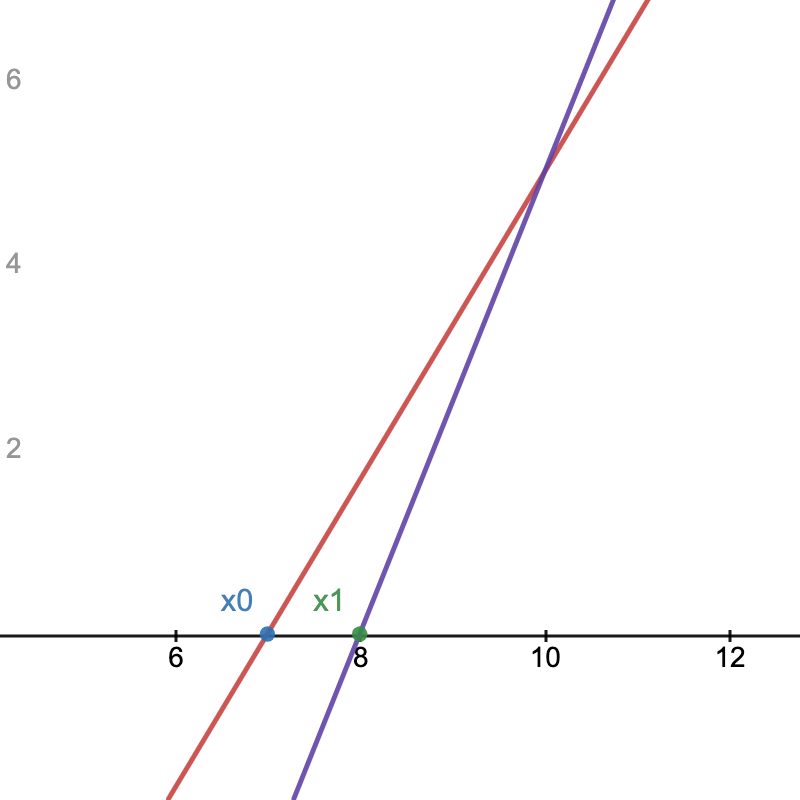
\includegraphics[width=\linewidth]{figures/shock_x1_x2_lt_half.png}
    \caption{$u(x_0) < u(x_1), u(x_0), u(x_1) \in (0, \frac{u_\infty}{2})$}\label{fig:shock_x1_x2_lt_half}
    \endminipage\hfill
    \minipage{0.32\textwidth}
    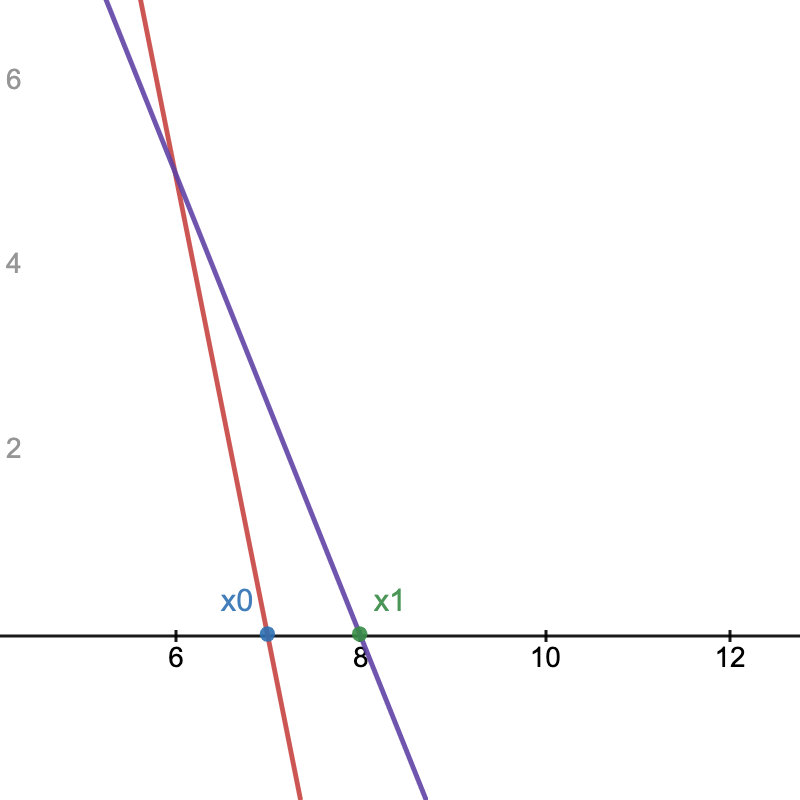
\includegraphics[width=\linewidth]{figures/shock_x1_x2_gt_half.png}
    \caption{$u(x_0) < u(x_1), u(x_0), u(x_1) \in (\frac{u_\infty}{2}, u_\infty)$}\label{fig:shock_x1_x2_gt_half}
    \endminipage\hfill
    \minipage{0.32\textwidth}%
    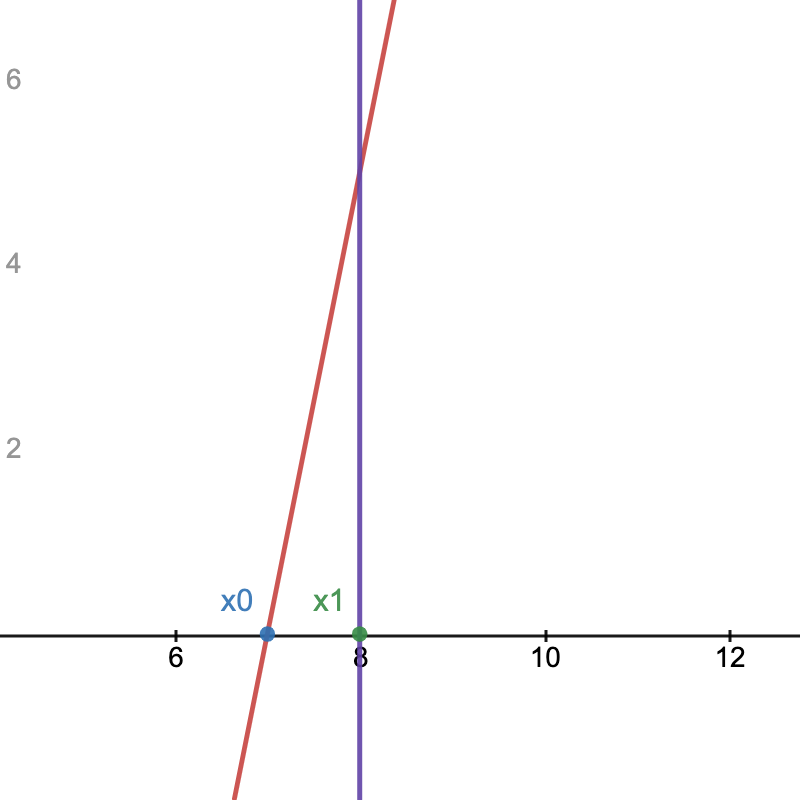
\includegraphics[width=\linewidth]{figures/shock_x1_eq_half.png}
    \caption{$u(x_0) < u(x_1), u(x_0) \in (\frac{u_\infty}{2}, u_\infty), u(x_1) = \frac{u_\infty}{2} $}\label{fig:shock_x1_eq_half}
    \endminipage
\end{figure}

Conversely, if the density of the initial condition is decreasing (i.e. when $x_0 < x_1 \implies u(x_0) < u(x_1)$), there are no shocks. See Figures  \ref{fig:no_shock_x1_x2_lt_half}, \ref{fig:no_shock_x1_x2_gt_half}, and \ref{fig:no_shock_x0_eq_half} for examples. 

\begin{figure}[!htb]
    \captionsetup{justification=centering}
    \minipage{0.32\textwidth}
    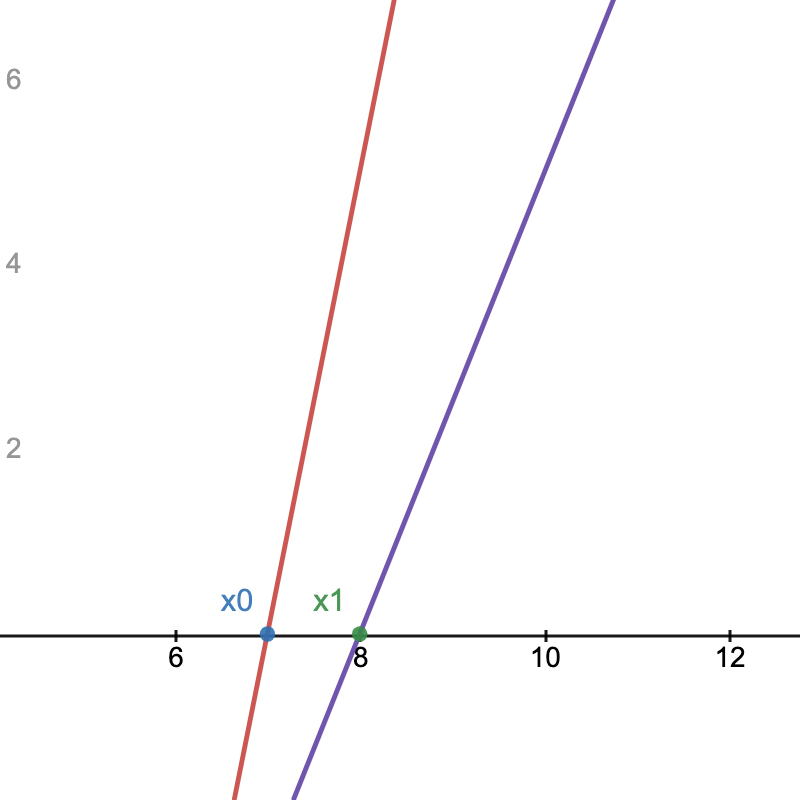
\includegraphics[width=\linewidth]{figures/no_shock_x1_x2_lt_half.png}
    \caption{$u(x_0) > u(x_1), u(x_0), u(x_1) \in (0, \frac{u_\infty}{2})$}\label{fig:no_shock_x1_x2_lt_half}
    \endminipage\hfill
    \minipage{0.32\textwidth}
    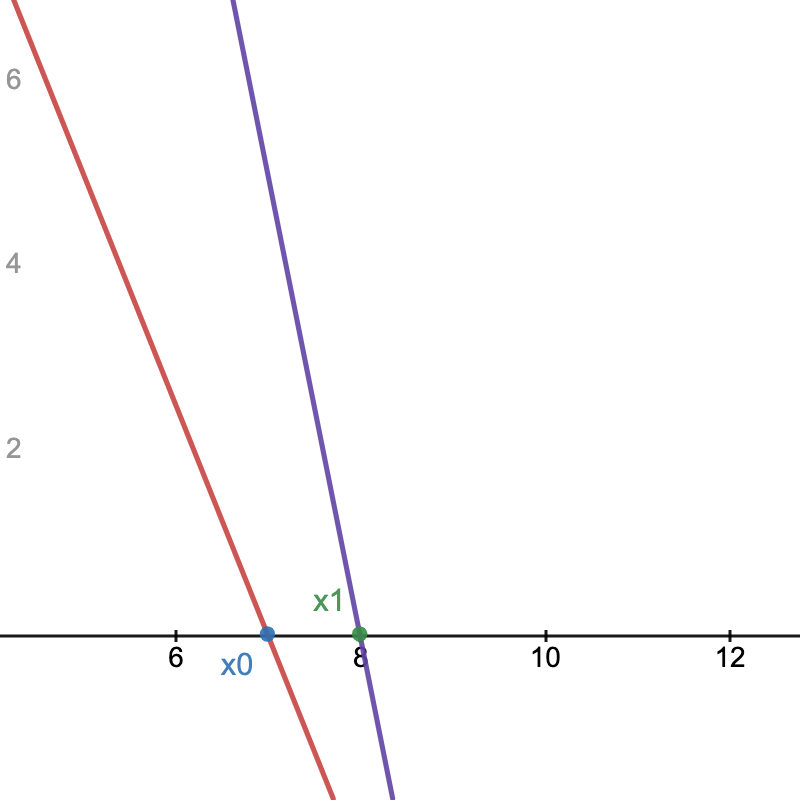
\includegraphics[width=\linewidth]{figures/no_shock_x1_x2_gt_half.png}
    \caption{$u(x_0) > u(x_1), u(x_0), u(x_1) \in (\frac{u_\infty}{2}, u_\infty)$}\label{fig:no_shock_x1_x2_gt_half}
    \endminipage\hfill
    \minipage{0.32\textwidth}%
    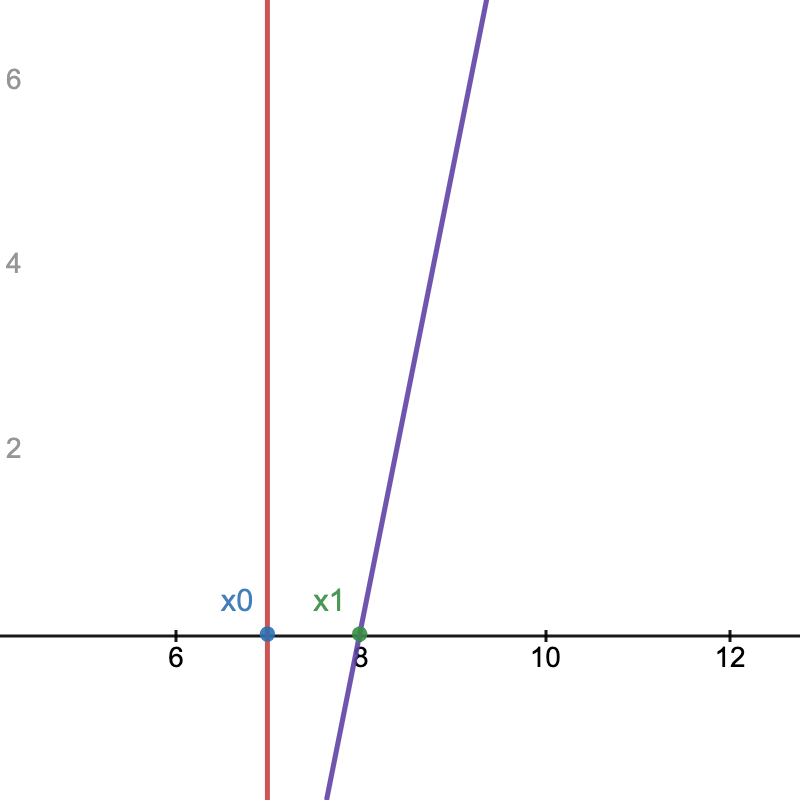
\includegraphics[width=\linewidth]{figures/no_shock_x0_eq_half.png}
    \caption{$u(x_0) < u(x_1), u(x_0) = \frac{u_\infty}{2},  u(x_0) \in (\frac{u_\infty}{2}, u_\infty) $}\label{fig:no_shock_x0_eq_half}
    \endminipage
\end{figure}

As a result of the pattern of characteristics, there are a lot of constraints as to the auxiliary conditions that we can feed our model given that we want well-defined solutions. As demonstrated above, no initial condition that is increasing will be well defined on any unbounded domain. Furthermore, note that if $u(x_0) \in (0, \frac{u_\infty}{2} )$, the slope of the characteristic will be positive, and in the case that $u(x_0) \in ( \frac{u_\infty}{2}, u_\infty )$ the slope will be negative. As a result, any left boundary that contains values in $( \frac{u_\infty}{2}, u_\infty )$ will overdetermine the initial condition, and likewise on the right boundary if there are values in $(0, \frac{u_\infty}{2} )$ the initial condition will also be overdetermined, and so we will not have a well-defined solution. 

%Write up numerical scheme with boundary conditions
%Try to figure out why sheme is unstable
%Apply to scenarios
%Note instability
%Try extending domain horizontally with an unrealistic rhs boundary condition OR have the cars come to red light (neumann)
%Figure out code for neumann b.c.
%
%try case 2 (will need to knock out diffusion term)
%
%combine simulations for case 3, TEEEHEHEEEEEEEEEEh
%
%Get this on overleaf
%Get riley and Laren's stuff  on here 

	\subsection{Introduction of Diffusion Term}
The introduction of the diffusion term then helps us work around some of the problems the characteristics run into. In addition, we were able to use boundary conditions that had discontinuities. If we had these with only an advection term, these discontinuities would simply be carried through the solution. However, with diffusion, these jumps tend to smooth out over time.

\subsection{Finite Difference Scheme}
We create a finite difference scheme of the equation by taking a forward time difference and a centered approximation of the spatial derivative. This gives us
\begin{align*}
u(x,t+\Delta t)=u(x,t)&+\Delta t[f(u(x,t))] \\
=u(x,t)&+V_{\infty}\Delta t\left[\epsilon u_{xx}-u_x\left(1-\frac{2u(x,t)}{u_{\infty}}\right)\right] \\
=u(x,t)&+\left[\frac{V_{\infty}\Delta t\epsilon}{(\Delta x)^2}(u(x+\Delta x, t)-2u(x,t)+u(x-\Delta x,t))\right] \\
&-\left[\frac{V_{\infty}\Delta t}{2\Delta x}\left(1-\frac{2u(x,t)}{u_{\infty}}\right)(u(x+\Delta x,t)-u(x-\Delta x,t)\right] \\
\end{align*}
%% Third Section
\section{Results of PDE Approach}

\section{Modeling Traffic Flow – SIR Approach}

\subsection{Governing Equations} 
We will use the equations 
\begin{align*}
    u_t + L(x, t) ( 1 - \frac{2n}{u_\infty} ) u_x = 0 
\end{align*}

and analyze this equation considering several cases and initial conditions. We have gotten this equation from the discussion on traffic in 8.1 of Volume 4, but have replaced the term $V_\infty$ with $L(x, t)$ where $L(x, t)$ will be defined as to simulate different stop light patterns. Other variables in this equation include $u_\infty$ which refers to the maximum density of cars at a given position. 

We expect to define the light equation $L$ as $L : \mathcal{R} \times \mathcal{R} \to [0, V_\infty]$. In situations where we are modeling cars getting going from stop as the light turn green, $L(x, t) = V_\infty$ and will be constant. In the situation where we model a red light turning on to stop oncoming traffic, we will examine different functions for $L(x, t)$ to see what kind of definition produces a realistic simulation of traffic flow. 

\subsection{Solutions}

We will attempt to solve these equations analytically, but will likely end up using numerical methods, especially as we get into weirder initial conditions (such as cars stopping at a red light). 

If we are successful at modeling cars starting and stopping at a light, we will attempt to model an intersection with cars coming and leaving in two perpendicular directions.

% %% First Section
% \section{Background/Motivation}
% Put your background motivation stuff here. You might reference something material here like \cite{ref1}.

% %% Second Section 
% \section{Modeling}
\subsection{SIR Details}
To better approximate a more complicated system with multiple interacting streams, we employed an SIR styled model. 

Structure
While there are many different traffic light intersections and variants, this model assumes a standard 4 way intersection with traffic coming from each of the cardinal directions (north, east, south, and west). Each direction has 3 streams of traffic, a turning left stream, a straight stream, and a right stream. 

\begin{figure}[htp]
    \centering
    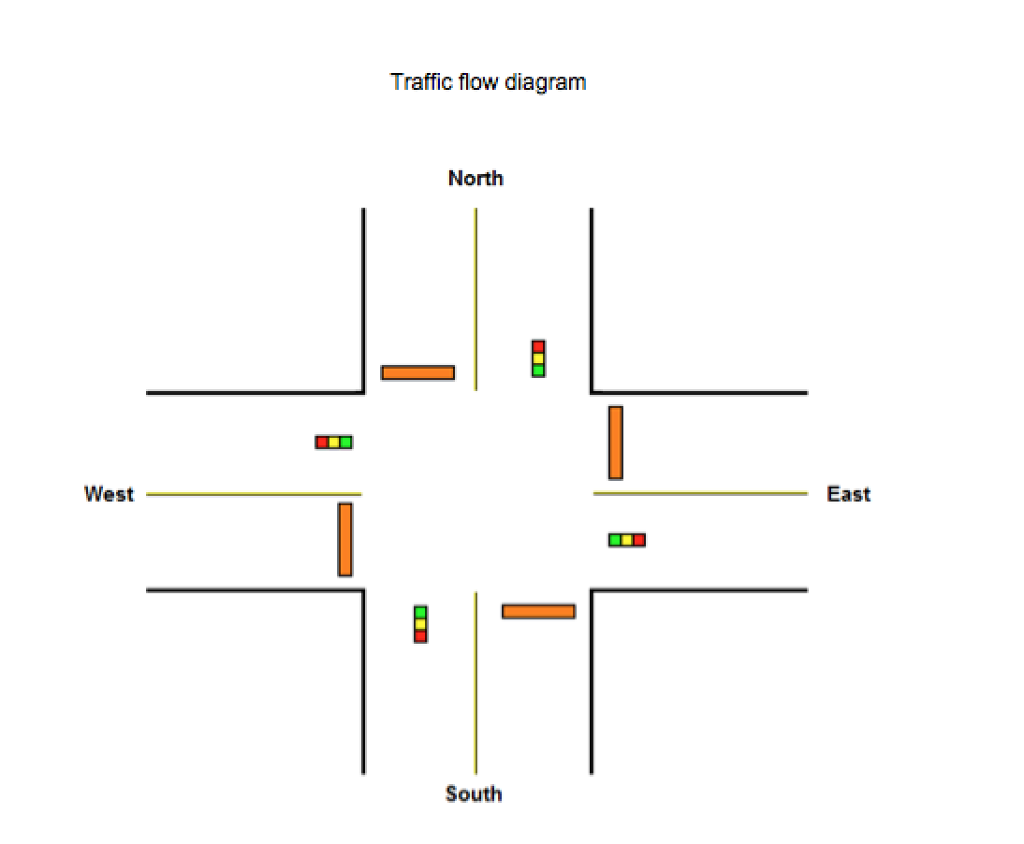
\includegraphics[width=11cm]{figures/TrafficDiagrampng.png}
    %  \caption{Traffic Flow Diagram}
    \label{fig:diagram}
\end{figure}

The change in the straight stream is only dependent on whether the light is red or green. The left stream is “unprotected”, meaning that the change in the left stream depends on whether the light is green and how much traffic is coming from the opposite straight stream. The right stream is free to turn at any time, and is only dependent on how much traffic is coming from the perpendicular straight stream.

\subsubsection{Implementation}

First, we define a light function. We want this function to be periodic and to move between 0 (red) and 1 (green). Rather than having one function that returns red for one direction and green for the other direction, we created two correlated functions that define the state of the light in the north-south direction and the east-west direction:

\[
\textrm{lightNS(t)} =
\begin{cases} 
    \sin(3t) & \frac{t}{ 2\pi} \mod 2 \pi\in [0, \frac{\pi}{6}) \\
    1 & \frac{t}{ 2\pi} \mod 2 \pi\in [\frac{\pi}{6},\frac{5\pi}{6}) \\
    \sin(3t) & \frac{t}{ 2\pi} \mod 2 \pi\in [\frac{5\pi}{6}, \pi) \\
    0 & \text{otherwise}
\end{cases}
\]




\begin{align*}
    \textrm{lightEW(t)} =
    \begin{cases} 
        -\sin(3t) & \frac{t}{2\pi} \mod 2 \pi \in [\pi,\frac{7\pi}{6} ) \\ 
        1 & \frac{t}{ 2\pi }\mod 2 \pi \in [\frac{7\pi}{6},11\frac{5\pi}{6} ) \\
        -\sin(3t) & \frac{t}{ 2\pi} \mod 2 \pi\in  [\frac{11\pi}{6}, 2 \pi) \\
        0 & \text{otherwise}
    \end{cases}
\end{align*}

Next, we define 12 different “bins”, one for each stream of our model (eg. North Forward), and then define the derivative of each bin:\\\\

\begin{flalign*}
    N_F'(t) = -1*\text{LightNS}(t)\\
    E_F'(t) = -1*\text{LightEW}(t)\\
    S_F'(t) = -1*\text{LightNS}(t)\\
    W_F'(t) = -1*\text{LightEW}(t)\\\\
    N_L'(t) = -1*\text{LightNS}(t)*(1+S_F'(t))\\
    E_L'(t) = -1*\text{LightEW}(t)*(1+W_F'(t))\\
    S_L'(t) = -1*\text{LightNS}(t)*(1+N_F'(t))\\
    W_L'(t) = -1*\text{LightEW}(t)*(1+E_F'(t))\\\\
    N_R'(t) = -1*W_F'(t)\\
    E_R'(t) = -1*S_F'(t)\\
    S_R'(t) = -1*E_F'(t)\\
    W_R'(t) = -1*N_F'(t)\\
\end{flalign*}



The definitions above assume constant base changes between all streams, that no new cars are entering the system, and that left turns have zero change whenever the cars coming straight are coming at full capacity. To account for these, we add some constants that allow for configuring the system:\\\\
\begin{flalign*}
    N_F'(t) = -1*c_f*\text{LightNS}(t)+add_f\\
    E_F'(t) = -1*c_f*\text{LightEW}(t)+add_f\\
    S_F'(t) = -1*c_f*\text{LightNS}(t)+add_f\\
    W_F'(t) = -1*c_f*\text{LightEW}(t)+add_f\\\\
    N_L'(t) = -1*c_l*\text{LightNS}(t)*((left\_turn\_gap\_c*c_f) + S_F'(t)) + add_l\\
    E_L'(t) = -1*c_l*\text{LightEW}(t)*((left\_turn\_gap\_c*c_f) + W_F'(t)) + add_l\\
    S_L'(t) = -1*c_l*\text{LightNS}(t*((left\_turn\_gap\_c*c_f) + N_F'(t)) + add_l\\
    W_L'(t) = -1*c_l*\text{LightEW}(t)*((left\_turn\_gap\_c*c_f) + E_F'(t)) + add_l\\\\
    N_R'(t) = -1*c_r*W_F'(t)+add_r\\
    E_R'(t) = -1*c_r*S_F'(t)+add_r\\
    S_R'(t) = -1*c_r*E_F'(t)+add_r\\
    W_R'(t) = -1*c_r*N_F'(t)+add_r\\
\end{flalign*}

\section{Results of SIR Approach}
Solutions to this system were calculated numerically with scipy.integrate.solve\_ivp.\\


\begin{figure}[h!]
    \centering
    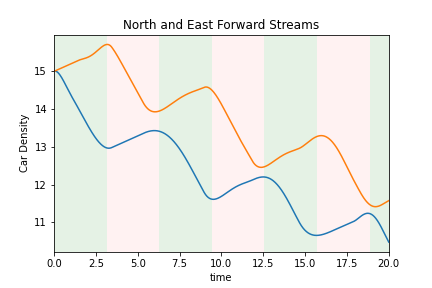
\includegraphics[width=12cm]{figures/NorthandEastForwardStreams.png}
    \label{fig:NorthandEastForwardStreams}
\end{figure}

Below we see the North and East forward streams, with the north-south light function shown with the alternating green and red zones. This model aligns with our expectations, with the number of cars waiting to go straight decreasing from the north when the light is green while the east stream accumulates more cars.\\

\begin{figure}[h!]
    \centering
    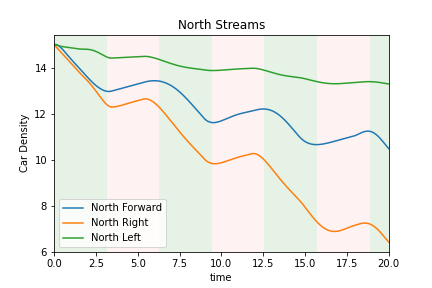
\includegraphics[width=12cm]{figures/NorthStreams.png}
    \label{fig:NorthStreams}
\end{figure}

Further below, we see the three different north streams. We see that while the light is green the forward and right streams change identically, however, the right stream continues to decrease during the transition from green to red. This again lines up with what we would expect from the rules of the system, as the right turn can continue to turn right up until cars start to flow forward from the east.\\

\begin{figure}[h!]
    \centering
    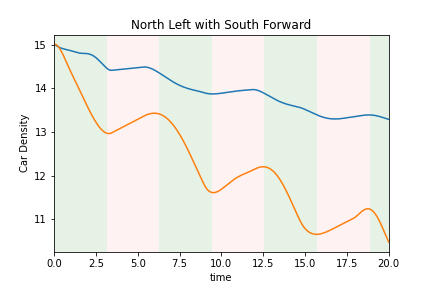
\includegraphics[width=12cm]{figures/NorthLeftwithSouthForward.png}
    \label{fig:NorthLeftwithSouthForward}
\end{figure}

Next we examine how a left turn interacts with the forward blocking stream. We see that the left turn has the sharpest decrease right before the light turns red. This is an interesting attribute of the model that lines up with how left turns behave in day to day life. Often, people waiting to turn left will creep into the intersection, then turn left as the light turns red and the oncoming traffic stops.\\

%%Fourth Section
\section{Conclusions}

\begin{thebibliography}{99}
\bibitem{ref1} First reference goes here
\end{thebibliography}

\end{document}
